\documentclass[11pt]{article}
\usepackage[toc,page]{appendix}
\RequirePackage{fix-cm}
\usepackage[utf8]{inputenc}
\usepackage[margin=1.5in]{geometry}
\usepackage[bottom, flushmargin]{footmisc}
\setlength{\footnotesep}{\baselineskip} % space between footnotes 
\setlength{\parindent}{0in} % space at start of paragraph
\setlength{\parskip}{0.14in} % space between paragraphs
\linespread{1.25}
\usepackage{titlesec}
\titlespacing\section{0pt}{0.21in}{0.03in}
\titlespacing\subsection{0pt}{0.21in}{0.01in}
\titlespacing\subsubsection{0pt}{0.21in}{0in}
\usepackage{marginnote}
\newcommand{\marnum}[1]{\reversemarginpar \marginnote{#1}[0.14in]}

% bibliography-related packages
\usepackage[superscript]{cite}
\bibliographystyle{unsrt}

% lists
\usepackage{enumitem} 
\newcommand{\bulletlabel}{\raisebox{0.2ex}{\small$\bullet$}}
\newlist{enumbul}{enumerate}{6}
\setlist[enumbul]{label=\bulletlabel, topsep=0pt, leftmargin=0.3in, rightmargin=0.3in}
\newlist{enumar}{enumerate}{6}
\setlist[enumar]{label=\arabic*$)$,topsep=0pt, leftmargin=0.3in, rightmargin=0.3in}

% packages vital for various things
\usepackage{hyperref}
\usepackage{comment} % commenting out a large chunk
\usepackage{enumitem} % lists
\usepackage{graphicx,nicefrac} % graphics, especially external ones
\graphicspath{ {dataviz/} }
\usepackage{amsmath} % writing math
\usepackage{amssymb} % writing symbols
\usepackage{amsthm}
\usepackage{bm}
\usepackage{float}
\usepackage{mathtools}
\usepackage{bigints}

% colors
\usepackage{tcolorbox}
\usepackage{color} % colors
\usepackage{xcolor, colortbl} % more control over colors
\newcommand{\red}[1]{\color{red}#1\color{black}}
\newcommand{\green}[1]{\color{green!80!black}#1\color{black}}
\newcommand{\blue}[1]{\color{blue}#1\color{black}}
\newcommand{\gray}[1]{\color{gray!80!black}#1\color{black}}
\newcommand{\black}[1]{\color{black}#1\color{black}}

\hypersetup{
	colorlinks,
	linkcolor=black, %internal links
	urlcolor=cyan,  % URLs
	citecolor= red, % references
	breaklinks=true
}

% for use in tables
\usepackage{multirow}
\usepackage{multicol}
\usepackage{array}
\usepackage{booktabs}
\newcommand\bstrut{\rule{0pt}{2.5ex}} % space before row
\newcommand\astrut{\rule[-1.25ex]{0pt}{0pt}} % space after row
\newcolumntype{L}[1]{>{\raggedright\let\newline\\\arraybackslash\hspace{0pt}}m{#1}}
\newcolumntype{C}[1]{>{\centering\let\newline\\\arraybackslash\hspace{0pt}}m{#1}}
\newcolumntype{R}[1]{>{\raggedleft\let\newline\\\arraybackslash\hspace{0pt}}m{#1}}

%miscellaneous
\newcommand{\ansm}[1]{\text{\framebox{\ensuremath{#1}}}}
\newcommand{\anst}[1]{\text{\framebox{#1}}}
\newcommand{\ie}[1][]{\textit{i.e.\ }#1}
\newcommand{\eg}[1][]{\textit{e.g.\ }#1}
\newcommand\pspace {\\[0.07in]}
\newcommand\ppspace {\\[0.14in]}
\newcommand{\logsep}{\begin{center}---------------\end{center}}

\def\highlight#1#2{
	\begin{centering}
		
		\vspace{1.2ex}
		\begin{minipage}{0.8\linewidth}
			\begin{tcolorbox}[boxsep = 3.3pt, boxrule=0.4pt, colback = white, colbacktitle=white, coltitle = black, colframe= black, title=\centering \textbf{#1}]
				\centering
				#2
			\end{tcolorbox}
		\end{minipage}
		\vspace{1.2ex}
		
	\end{centering}
}

\begin{document}
\pagenumbering{gobble}
\def\acronymend{MECo}
\def\acronym{\acronymend\space}

\phantom{Thevesh}

\vfill

\begin{center}
	\begin{minipage}{0.88\linewidth}
		\begin{center}
			\LARGE
			The Malaysian Election Corpus (\acronymend):\\Federal and State-Level Election Results\\from 1955 to 2025 \\[0.21in]
			\Large
			Thevesh Thevananthan\\[0.15in]  % ← Author name inserted here
		\end{center}
		\large 
		Empirical research and public knowledge on Malaysia's elections have long been constrained by a lack of high-quality open data, particularly in the absence of a Freedom of Information framework. We introduce the Malaysian Election Corpus (MECo; \href{https://electiondata.my}{ElectionData.MY}), an open-access panel database covering all federal and state general elections from 1955 to the present, as well as by-elections from 2008 onward. MECo includes candidate- and constituency-level results for nearly 10,000 contests across seven decades, standardised with unique identifiers for candidates, parties, and constituencies. The database also provides summary statistics on electorate size, voter turnout, rejected votes, and unreturned ballots. This is the most well-curated publicly available data on Malaysian elections, and will unlock new opportunities for research, data journalism, and civic engagement.
	\end{minipage}
\end{center}

\vfill

\phantom{Word Count:}

\newpage
\pagenumbering{arabic}

\def\TOTALBALLOTS{25,552}
\def\TOTALCONTESTS{9,705}
\def\TOTALPARTIES{99}
\def\TOTALCONTESTSSTATE{6,935}
\def\TOTALCONTESTSFEDERAL{2,770}
\def\TOTALELECTIONS{16}

\section*{Background \& Summary}
Malaysia's electoral history is among the most dynamic in Southeast Asia, encompassing \TOTALCONTESTSFEDERAL\space federal general elections and \TOTALCONTESTSSTATE\space state general elections (Figure \ref{fig:elections}), as well as hundreds of off-cycle by-elections across a multiethnic, multi-party system. Furthermore, Malaysia offers significant scope for the study of democratisation, having experienced its first change of ruling party in 2018, and its first ever hung Parliament as recently as 2022. However, conducting empirical studies of Malaysian elections is challenging due to the lack of a comprehensive, standardised, and publicly available dataset that provides a single source of truth for scholars. The Election Commission (EC) does not publish machine-readable open data which abides by best practices for data sharing, preferring instead to limit citizens to searching up isolated results\cite{mysprsemak}. Slightly richer information is available via gazetted election results published as subsidiary legislation\cite{lompub}, but these are published in PDF format only. The lack of a Freedom of Information Act further complicates efforts to acquire electoral returns.

\begin{figure}[htbp]
	\makebox[\textwidth][c]{
		\begin{minipage}{1.15\textwidth}
			\centering
			\caption{Federal and state general election years}
			\vspace{0.14in}
			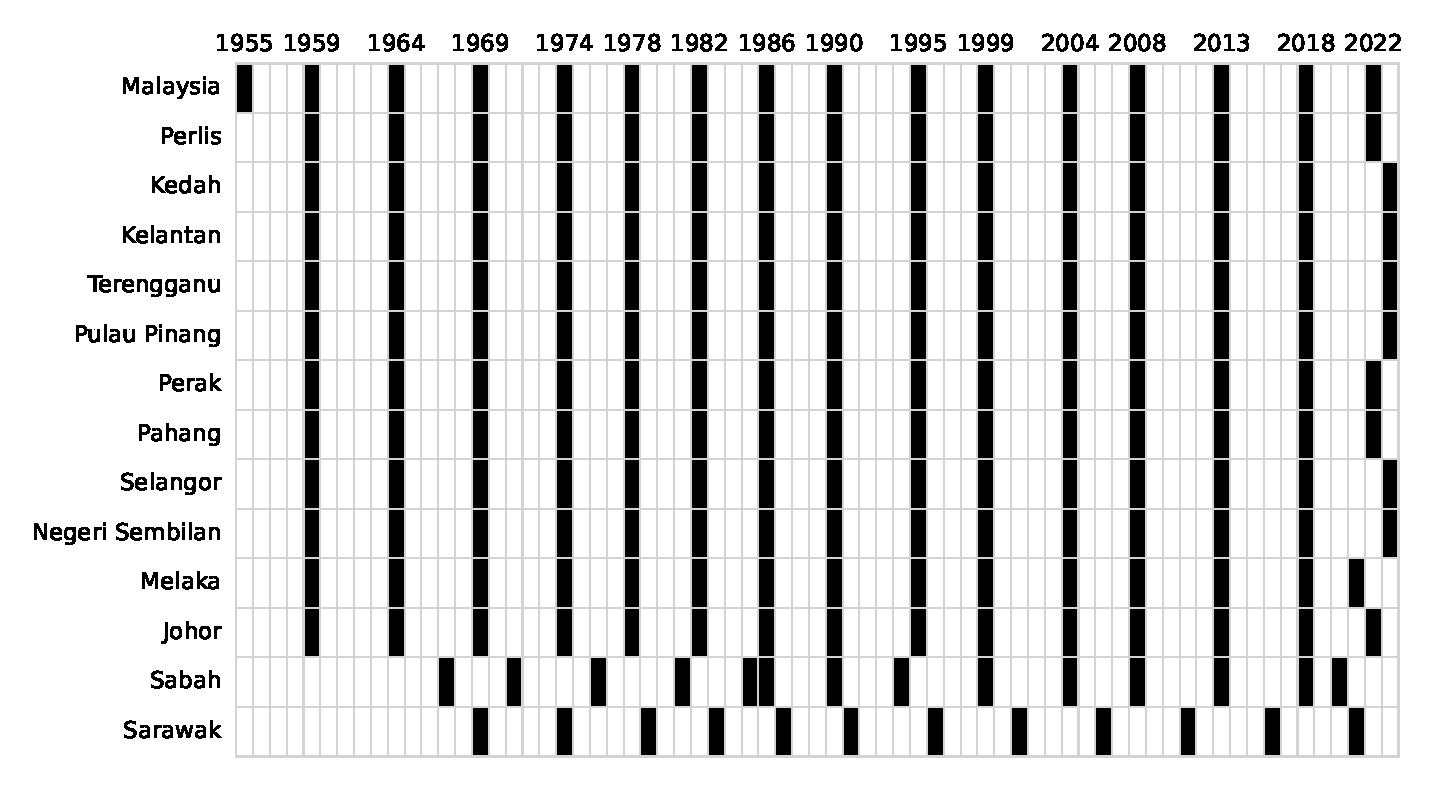
\includegraphics[width=\linewidth]{dataviz/heatmap_elections.eps}
			\label{fig:elections}
		\end{minipage}
	}
\end{figure}

Amidst this paucity of data, global initiatives such as the Constituency-Level Elections Archive (CLEA)\cite{clea} provide immensely valuable cross-country coverage, including for Malaysian elections. However, they generally focus on federal contests, and within that scope, only on the number of votes won by each candidate (thus omitting information such as the electorate size, voter turnout,unreturned ballots, rejected votes, etc). Similarly, international turnout or election integrity datasets\cite{icoma2023urnout,norris2014integrity} capture only high-level national indicators. Locally, a number of news and civil society organisations\cite{undiinfo,ge15sinar,tindakgithub} compile election data to varying degrees of completeness and quality, but these efforts -- while laudable for their public service, and valuable as a stopgap measure -- typically lack proper data hygiene and standardisation, and are not subjected to systematic validation and review, thus limiting their usefulness for rigorous empirical research and long-term preservation.

In this paper, we address this gap by providing the first comprehensive open database of Malaysian election results at the federal and state level -- we intend for this to be a living resource which provides the go-to empirical foundation for research and journalism on Malaysian elections. The database covers \textit{all} general elections since the pre-independence general election in 1955, and 115 by-elections held since 2008. In total, it records \TOTALBALLOTS\space candidates representing \TOTALPARTIES\space political parties in \TOTALCONTESTS\space unique electoral contests from 1955 to 2025. The dataset comprises two main components:
\begin{enumbul}
\item \textbf{Ballots}: The final results for each state legislative assembly constituency (DUN) and federal Parliament constituency (Parliament), with the number of votes received by each candidate.
\item \textbf{Summaries}: The electorate size, ballots issued, unreturned ballots, and votes rejected in each constituency. For each constituency, we also derive the margin of victory (majority), voter turnout rate, vote rejection rate, unreturned ballot rate, and majority as a share of valid votes.
\end{enumbul}

Furthermore, our database offers three key advantages built on the use of unique identifiers (UIDs). First, we encode a UID for each candidate, thus allowing the tracking of a single individual across time, even if they run under different political parties or change the name which they use in public life; this is especially important in Malaysia, because politicians are not required to use their official name on electoral ballots. Second, we encode a UID for each party, allowing for tracking of party evolution, such as the expansion of the Alliance Party (\textit{Parti Perikatan}) into the National Front (\textit{Barisan Nasional}). Third, we provide a lookup for each unique date-state-constituency combination, allowing for the creation of geospatial lineage and tracking of changes in constituency names. In general, the use of UIDs makes our database highly extensible -- a deliberate choice to help other scholars seamlessly build on our work by creating new lookups, rather than altering core datasets.

To the best of our knowledge, no comparable database exists. As a living resource, this paper lays the foundation for future data curation, as well as research into areas like malapportionment, gerrymandering, local-level voting patterns, and the spatial dynamics of political competition. We also hope that \acronym will serve as a catalyst for broader collaborations between academics, civil society, journalists, and election observers, supporting both scholarly inquiry and public accountability.

Finally, we note that while our work is the first of its kind for Malaysian elections, it follows a growing body of recent academic work focused on compiling and curating country-specific election data for reuse.\cite{perez2021spanish,baltz2022american,de2023american,calderon2025electoral,heddesheimer2025gerda,jensenius2017studying} By situating \acronym within this emerging tradition of high-quality electoral data curation, we contribute to the rapidly-improving global infrastructure of comparative political research. This work reflects a commitment to transparency, reproducibility, and the democratisation of access to electoral information.

\section*{Methods}
There are three sources of data we used to construct our database:
\begin{enumar}
\item Physical post-election reports\cite{ge00report,ge01report,ge02report,ge03report,ge04report,ge05report,ge06report,ge07report,ge08report,ge09report,ge10report,ge11report,ge12report,ge13report,sabah1967report,sabah1971report,sabah1976report,sabah1981report,sabah1985report,sabah1986report,sabah1990report,sabah1994report,sabah1999report,sarawak1979report,sarawak1983report,sarawak1987report,sarawak1991report,sarawak1996report,sarawak2001report,sarawak2006report,kelantan1978report}.
\item Gazetted election results published as subsidiary legislation\cite{lompub}.
\item Digital results published officially by the EC via a dashboard\cite{mysprsemak}.
\end{enumar}
To enable checking and validation, we made images of the post-election reports and PDFs of the gazetted election results (sources 1 and 2) available via this \href{https://kongsi.la/tmECWBT}{anonymous Dropbox link}. We constructed \acronym beginning with federal general elections, then state general elections, and finally by-elections. This is because state legislative assembly constituencies (DUNs) must lie completely within the boundaries of a federal parliamentary constituency (Parliament), so it was sensible to begin with the superset. By-elections coming last is an intuitive choice, since a by-election must follow a general election by definition; validation of by-election data is therefore dependent on having complete federal and state-level results.

\subsection*{Federal General Elections}

\begin{figure}[htbp]
	\makebox[\textwidth][c]{
		\begin{minipage}{1.2\textwidth}
			\centering
			\caption{Federal election coverage (number of seats)}
			\vspace{0.14in}
			\includegraphics[width=1\linewidth]{dataviz/heatmap_seats_federal.eps}
			\label{fig:federal_coverage}
		\end{minipage}
	}
\end{figure}

For the 3 elections after 8th March 2008 (Figure \ref{fig:federal_coverage}), official results are available digitally via the aforementioned dashboard, in a manner that enabled us to directly scrape the results, albeit with the trial and error generally required for frontend web scraping. Where unavailable (all 13 elections prior to and including the 2008 federal general election), we manually (i.e.\ by hand) digitised the data from the aforementioned post-election reports and gazetted results. We made a deliberate methodological choice to avoid the use of optical character recognition (OCR) and PDF parsing tools after initial experimentation revealed an average error rate of approximately 10\%, primarily due to frequent changes in formatting and layout, even within the same document. We considered this to be unacceptably high for a resource intended to serve as a single source of truth. Moreover, the downstream process of error detection and correction proved to be more time-consuming and error-prone than simply transcribing the data by hand, especially given the relatively manageable size of this data (\TOTALBALLOTS\space ballots across \TOTALCONTESTS\space electoral contests). 

As a result, all records acquired from physical books or PDFs were transcribed by hand. The Technical Validation section further explains why the way in which Malaysia reports election results made it possible for us to do this with near-total confidence in the accuracy of the final product.

Records for seats in Peninsular Malaysia begin in 1955, while records for seats in Sabah and Sarawak begin in 1969. Although there was a federal general election in 1964, one year after Sabah and Sarawak (and Singapore) joined then-Malaya to form the Federation of Malaysia in 1963, seats in Sabah and Sarawak were not contested since the transition agreement allowed their respective state legislatures to appoint (and not elect) their representatives to the federal Parliament.\cite{means1991malaysia} There are no records for Singapore, which was not contested in the 1964 general election for the same reason as Sabah and Sarawak, and which exited the Federation prior to the next federal general election in 1969.

\subsection*{State General Elections}

For state-level general elections, we compiled data using the same three primary sources: post-election reports published by the EC, gazetted election results, and digital results where available. The same combination of web scraping and manual digitisation used for federal general elections was applied here.

For states in Peninsular Malaysia, records begin in 1959, when general elections for all 13 state legislative assemblies were held concurrently with the federal general election. For Sabah and Sarawak, records begin in 1967 and 1969 respectively, the years of the first state general elections held after the formation of the Federation of Malaysia. In all, \acronym contains records for 15 elections for all states in Peninsular Malaysia, 14 elections for Sabah, and 12 for Sarawak (Figure \ref{fig:state_coverage}). The reason for the discrepancy between the number of observations for Sabah and Sarawak is that there were two instances in Sabah's electoral history where state general elections were held in relatively quick succession. The first was in 1986, when Sabah went to the polls just one year after the previous state general election due to increasing civil and political instability\cite{yusoff2001sabah}. The second was in 2020, when Sabah held a state general election two years after the watershed election of 2018 due to a collapse of the state government\cite{lee2020collapse}.

\begin{figure}[htbp]
	\makebox[\textwidth][c]{
		\begin{minipage}{1.2\textwidth}
			\centering
			\caption{State election coverage (number of seats)}
			\vspace{0.14in}
			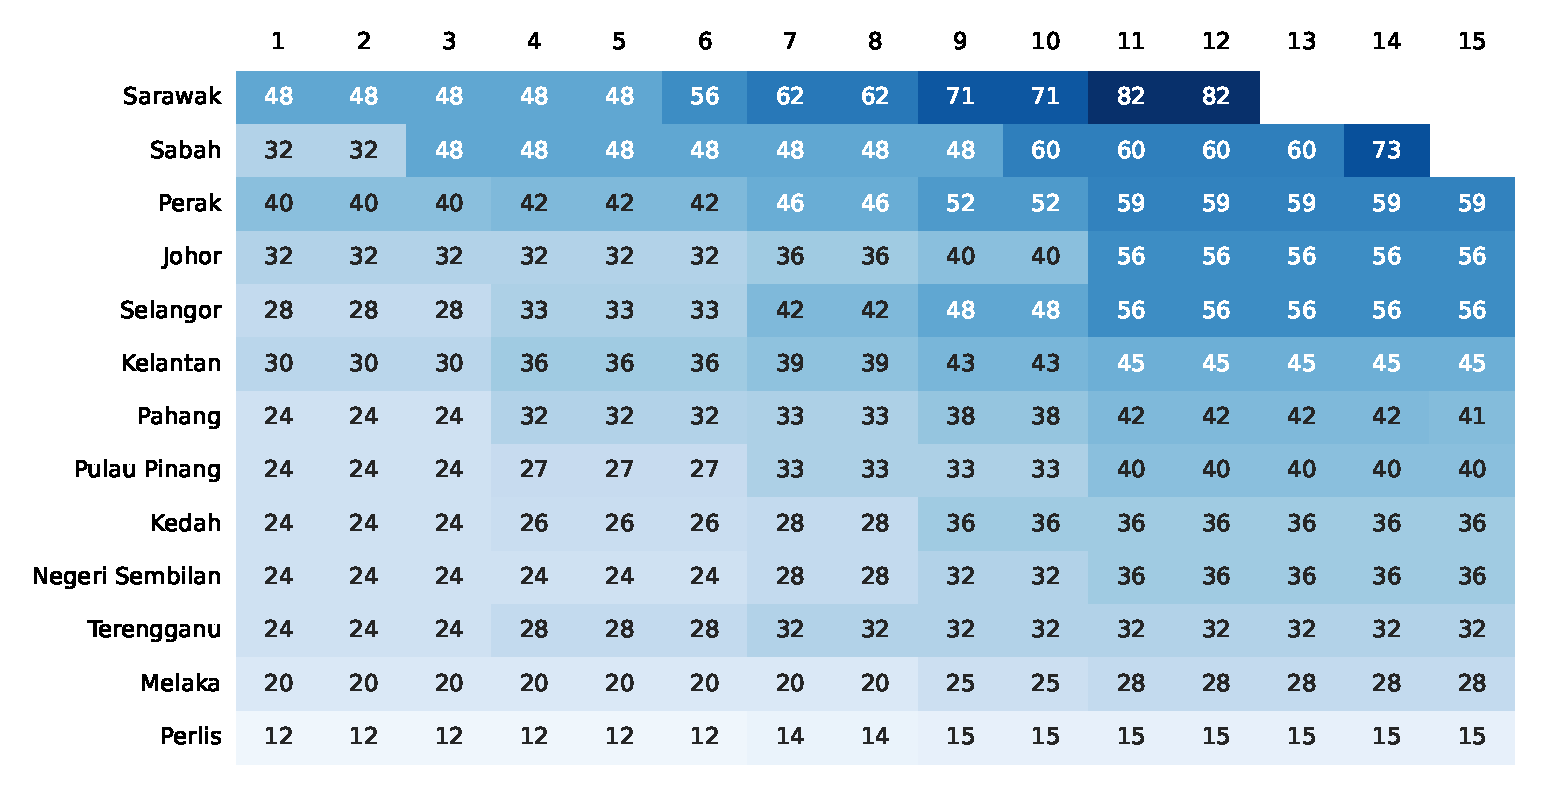
\includegraphics[width=1\linewidth]{dataviz/heatmap_seats_state.eps}
			\label{fig:state_coverage}
		\end{minipage}
	}
\end{figure}

\subsection*{By-Elections}

The by-elections dataset covers all Parliament and DUN by-elections held since the 12th federal general election in 2008, totaling 115 contests as of end-April 2025 (Figure \ref{fig:by_coverage}). Unlike for general elections, we could not locate any systematically compiled post-election reports or gazetted results for older by-elections. As a result, we relied solely on digital results made available via the EC's official website, which only covers by-elections since 2008. These digital records were scraped and harmonised with the same schema used for general elections.

\begin{figure}[htbp]
	\centering
	\caption{Byelection coverage (number of elections)}
	\vspace{0.14in}
	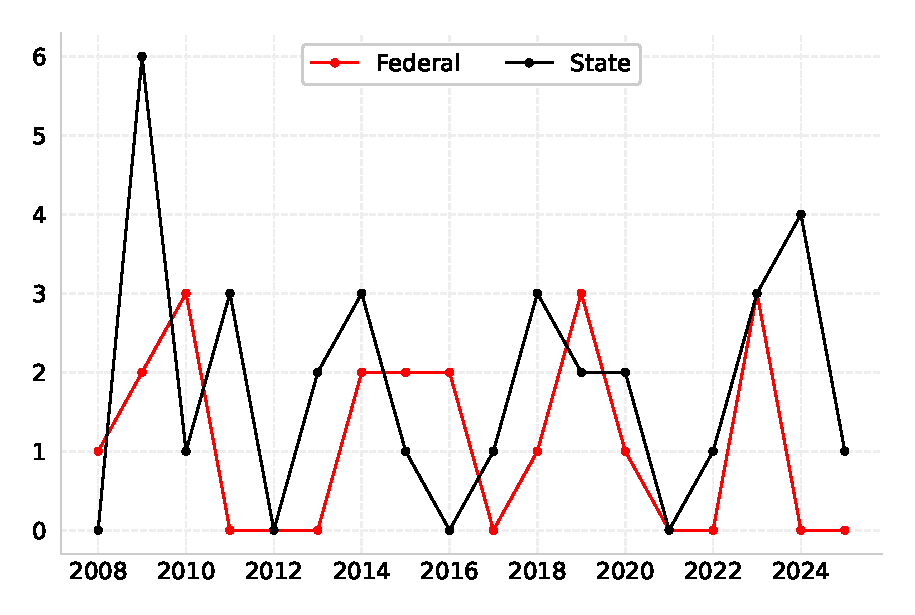
\includegraphics[width=0.8\linewidth]{dataviz/timeseries_byelections.eps}
	\label{fig:by_coverage}
\end{figure}

We plan to expand the dataset to include an exhaustive record of previous by-elections once we are able to acquire a reliable source, likely via a combination of EC reports and Hansards from Parliament and State Legislative Assemblies. However, we made the decision not to delay the dissemination of the primary \acronym datasets any further. Given that the most recent three election cycles are already fully covered, the exclusion of older by-elections is likely negligible for almost all prospective users.

\subsection*{Unique Identifier (UID) Generation}

The database incorporates unique identifiers (UIDs) for parties and candidates to enable consistent tracking across elections and to facilitate longitudinal analysis. Additionally, constituency harmonisation is handled through a pragmatic approach that avoids imposing subjective judgments about boundary changes.

\textbf{Parties.}
Party UIDs were generated manually, given that the total number of distinct parties in the dataset is relatively small (approximately 100). No historical harmonisation was conducted for parties that evolved or rebranded over time. For example, \textit{Parti Perikatan} and \textit{Barisan Nasional} are assigned separate UIDs, even though the latter is widely regarded as the successor to the former. This approach maintains full historical fidelity and allows users to apply their own ex-post harmonisation logic.

\textbf{Candidates.}
Candidate UIDs were generated through a combination of fuzzy matching and manual correction, enabling the tracking of individual candidates across multiple elections even when their names changed in spelling, formatting, or title usage over time. This is particularly important in the Malaysian context, where candidates frequently acquire new honorifics, adopt different formatting conventions, or have minor spelling variations across election cycles. Two illustrative examples highlight the complexity of this task. 8-time Parliamentarian \textbf{Rafidah Aziz} appeared on ballots across 8 elections in forms including:

\begin{centering}

Rafidah Aziz\\
Rafidah Bt. Ab. Aziz\\
Rafidah Bt. Abdul Aziz\\
Datuk Seri Rafidah Aziz

\end{centering}

Another 8-time Parliamentarian \textbf{Samy Vellu A/L Sangalimuthu} appeared on ballots across 9 elections with variations such as:

\begin{centering}

S. Samy Vellu\\
Datuk Seri Samy Vellu\\
S. Samy Vellu A/L Sangalimuthu\\
Dato' S. Samy Vellu A/L Sangalimuthu

\end{centering}
Through careful matching and correction, we assigned a single UID to all instances of a candidate to support longitudinal analysis.

\textbf{Constituencies.}
We deliberately avoided assigning UIDs to constituencies. Instead, we rely on the intrinsic uniqueness of the \texttt{date-state-constituency} combination, which guarantees that each contest is uniquely identifiable within its context (since no two constituencies within the same state can have the same name in the same election). A left join on these three fields suffices to generate a lookup table via which additional data can be merged. To aid users in harmonising constituencies across elections, we provide a field called \texttt{area\_name}, which standardises name changes and spelling variations across time. Examples include:
\begin{align*}
\text{Temerluh} &\rightarrow \space \text{Temerloh}\\ 
\text{Telok Anson} &\rightarrow \space \text{Teluk Intan}\\
\text{Bagan Datoh} \rightarrow \space \text{Bagan}&\text{ }\text{Datok} \rightarrow \space \text{Bagan Datuk}
\end{align*}
We do not currently implement harmonisation for changes involving boundary adjustments or the creation of new constituencies. For example, although the seat of Bayan Baru in Penang was carved out of Balik Pulau, we do not merge or tag these together because Balik Pulau remains an active seat name today, and such harmonisation would require subjective judgment. Our aim is to provide a flexible foundation that allows users to apply their own harmonisation strategies according to their specific research needs.

\section*{Data Records}
The data records supporting this paper are available through multiple platforms to facilitate access, transparency, and long-term preservation:

\begin{enumbul}
\item \textbf{Harvard Dataverse}\\
All primary datasets (Table \ref{tab:data_records}) are published and versioned on Harvard Dataverse at \url{https://doi.org/10.7910/DVN/O4CRXK}. This serves as the canonical archive for replication and reuse.

\item \textbf{GitHub}\\
The full source code used to process, compile, and validate the data is publicly available under a CC0 license at \url{https://github.com/Thevesh/paper-malaysian-election-corpus}. This repository also contains all files made available on Harvard Dataverse in both CSV and the highly efficient Parquet format, as well as raw source files split by state and election type.

\item \textbf{Companion Website}\\
The data can be interactively explored via \href{https://electiondata.my}{ElectionData.MY}. In addition to making the data accessible to non-technical users, the site is intended to serve as the primary channel for continuous updates and future enhancements to \acronymend.
\end{enumbul}

\begin{table}[H]
	\def\arraystretch{1.3}
	\centering
	\caption{Description of primary datasets}
	\label{tab:data_records}
	\vspace{0.14in}
	\begin{tabular}{L{0.29\linewidth}L{0.69\linewidth}}
	\toprule
	\textbf{Filename} & \textbf{Description} \\
	\midrule
	\texttt{consol\_ballots} & Candidate-level results for all federal and state elections \\
	\texttt{federal\_ballots} & Subset of \texttt{consol\_ballots} for federal general elections \\
	\texttt{state\_ballots} & Subset of \texttt{consol\_ballots} for state general elections \\
	\texttt{byeelection\_ballots} & Subset of \texttt{consol\_ballots} for by-elections \\ \hline
	\texttt{consol\_summary} & Summary statistics for all federal and state elections \\
	\texttt{federal\_summary} & Subset of \texttt{consol\_summary} for federal general elections \\
	\texttt{state\_summary} & Subset of \texttt{consol\_summary} for state general elections \\
	\texttt{byeelection\_summary} & Subset of \texttt{consol\_summary} for by-elections \\
	\texttt{lookup\_candidates} & Standardised candidate names \\
	\texttt{lookup\_parties} & Standardised party names and abbreviations \\
	\texttt{lookup\_dates} & Election dates, by state and election type \\
	\texttt{lookup\_seats} & Standardised constituency names \\
	\hline
	\texttt{logs/corrections} & Log of manual corrections applied to ballot issued counts to ensure consistency as described in the Technical Validation section \\
	\bottomrule
	\end{tabular}
\end{table}

Table \ref{tab:ballots_structure} describes the structure of \texttt{*\_ballots} files, while Table \ref{tab:summary_structure} describes the structure of \texttt{*\_summary} files.

\begin{table}[ht]
	\def\arraystretch{1.3}
	\centering
	\caption{Structure of all \texttt{*\_ballots} files}
	\label{tab:ballots_structure}
	\vspace{0.14in}
	\begin{tabular}{L{0.29\linewidth}L{0.69\linewidth}}
	\toprule
	\textbf{Variable} & \textbf{Description} \\
	\midrule
	\texttt{date} & Date of the election (YYYY-MM-DD) \\
	\texttt{election} & Election name (e.g., GE-14, SE-10, BY-ELECTION) \\
	\texttt{state} & State in which the constituency is located \\
	\texttt{seat} & Code and full name of the seat (e.g., P.052 Bayan Baru) \\
	\texttt{ballot\_order} & Order in which the candidate appeared on the ballot \\
	\texttt{name} & Candidate name as it appeared on the ballot paper \\
	\texttt{candidate\_uid} & Unique identifier for the candidate \\
	\texttt{party} & Party name as it appeared on the ballot paper \\
	\texttt{party\_uid} & Unique identifier for the party \\
	\texttt{votes} & Number of valid votes received by the candidate \\
	\texttt{votes\_perc} & Share of valid votes received by the candidate (\%) \\
	\texttt{result} & Outcome (won, won uncontested, lost, lost deposit) \\
	\bottomrule
	\end{tabular}
\end{table}

\begin{table}[ht]
	\def\arraystretch{1.3}
	\centering
	\caption{Structure of all \texttt{*\_summary} files}
	\label{tab:summary_structure}
	\vspace{0.14in}
	\begin{tabular}{L{0.35\linewidth}L{0.65\linewidth}}
	\toprule
	\textbf{Variable} & \textbf{Description} \\
	\midrule
	\texttt{date} & Date of the election (YYYY-MM-DD) \\
	\texttt{election} & Type of election (e.g., GE-14, SE-10, BY-ELECTION) \\
	\texttt{state} & State in which the constituency is located \\
	\texttt{seat} & Full name of the seat (e.g., P.049 Tanjong) \\
	\texttt{voters\_total} & Total number of registered voters \\
	\texttt{ballots\_issued} & Number of ballots issued \\
	\texttt{ballots\_not\_returned} & Number of ballots not returned (often postal votes) \\
	\texttt{votes\_rejected} & Number of rejected (spoiled) votes \\
	\texttt{votes\_valid} & Number of valid votes \\
	\texttt{majority} & Margin of victory between the top two candidates \\
	\texttt{voter\_turnout} & Ballots issued as a share of registered voters (\%) \\
	\texttt{majority\_perc} & Majority as a share of valid votes (\%) \\
	\texttt{votes\_rejected\_perc} & Rejected votes as a share of ballots returned (\%) \\
	\texttt{ballots\_not\_returned\_perc} & Unreturned ballots as a share of ballots issued (\%) \\
	\bottomrule
	\end{tabular}
\end{table}
	

\section*{Technical Validation}
There are four components of the database which require validation: Numerical data, candidate names, party names, and constituency names. 

For numerical data, the way in which Malaysia reports election results makes a unique form of validation possible. First, we define the following variables:
\begin{align*}
	I &= \text{Ballots Issued} \\
	U &= \text{Unreturned Ballots} \\
	R &= \text{Votes Rejected} \\
	V_i &= \text{Valid Votes for Candidate } i
\end{align*}
For a given contest involving $N$ candidates, the following relationship must hold:
\begin{align}
	\label{eq:validation}
	I - U - R = \sum_{i=1}^{N} V_i
\end{align}
In plain language, the implied number of valid votes must be equal to the sum of votes received by all candidates. Because $I$, $U$, $R$, and $V_i$ are (and have been) reported separately in all historical election reports and gazetted results, we can leverage this relationship as an almost-foolproof way to validate the accuracy of our manual data entry process. For transparency, we detected and corrected errors for 82 out of \TOTALCONTESTS\space contests, implying an error rate of 0.84\%, which is significantly lower than the 10\% error rate we encountered in our initial OCR experiments. Importantly, these errors are detectable and fixable, and come without the additional overhead of correcting errors in text data; our familiarity with local geography, politicians, and culture enabled us to transcribe text data rapidly and accurately.

This validation procedure also revealed 115 contests (excluding the 2006 Sarawak state general election, which did not report $I$, $U$, or $R$) for which the data was digitised accurately based on our source material, but which nevertheless failed to satisfy Equation (\ref{eq:validation}). These errors presumably occurred due to mistakes in data entry which were not caught and corrected during the original publication process. In order to ensure a clean dataset, we applied a standard correction -- for all 115 contests failing validation, we adjust the number of ballots issued (as documented in \texttt{corrections.csv}) such that Equation (\ref{eq:validation}) holds. We choose \texttt{ballots\_issued} as the variable to adjust for two reasons. First, until the 1989 amendment of the Elections (Conduct of Elections) Regulations 1981 (implemented at the 1989 federal general election), the number of unreturned ballots was not reported. Second, because the number of rejected votes is very small relative to the number of ballots issued, using rejected votes as the adjusted variable would have resulted in a much larger correction in percentage terms -- specifically, the correction would have required a 20\% change to the number of rejected votes on average (with several exceeding 50\%), relative to a 0.6\% change to the number of ballots issued (with only one above 5\%, and none above 20\%).

\begin{figure}[htbp]
	\centering
	\caption{Error rate in general election years}
	\vspace{0.14in}
	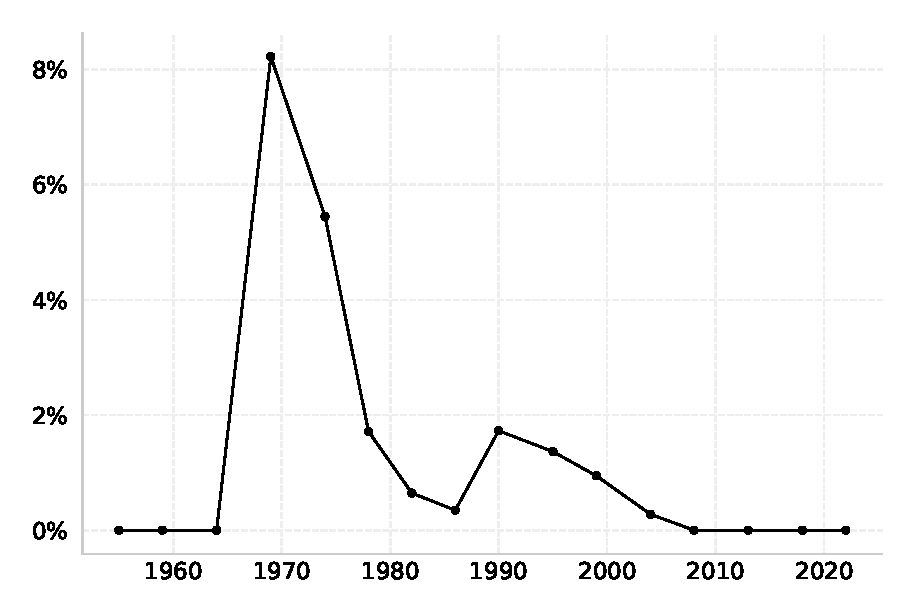
\includegraphics[width=0.7\linewidth]{dataviz/timeseries_error_rate.eps}
	\label{fig:error_rate}
\end{figure}


An interesting trend emerges when we plot the error rate arising from these 115 contests (Figure \ref{fig:error_rate}). The error rate was 0\% up to 1964, but spiked to nearly 8\% in 1969, when elections were severely disrupted by the Emergency. By 1978, error rates stabilised below 2\%, and have been constant at 0\% since 2008. We posit that this reflects general improvements in data management technology over the decades; we do not have a clear explanation for why no errors were made up to 1964.

\begin{figure}[ht]
	\centering
	\caption{Histogram of derived variables}
	\vspace{0.14in}
	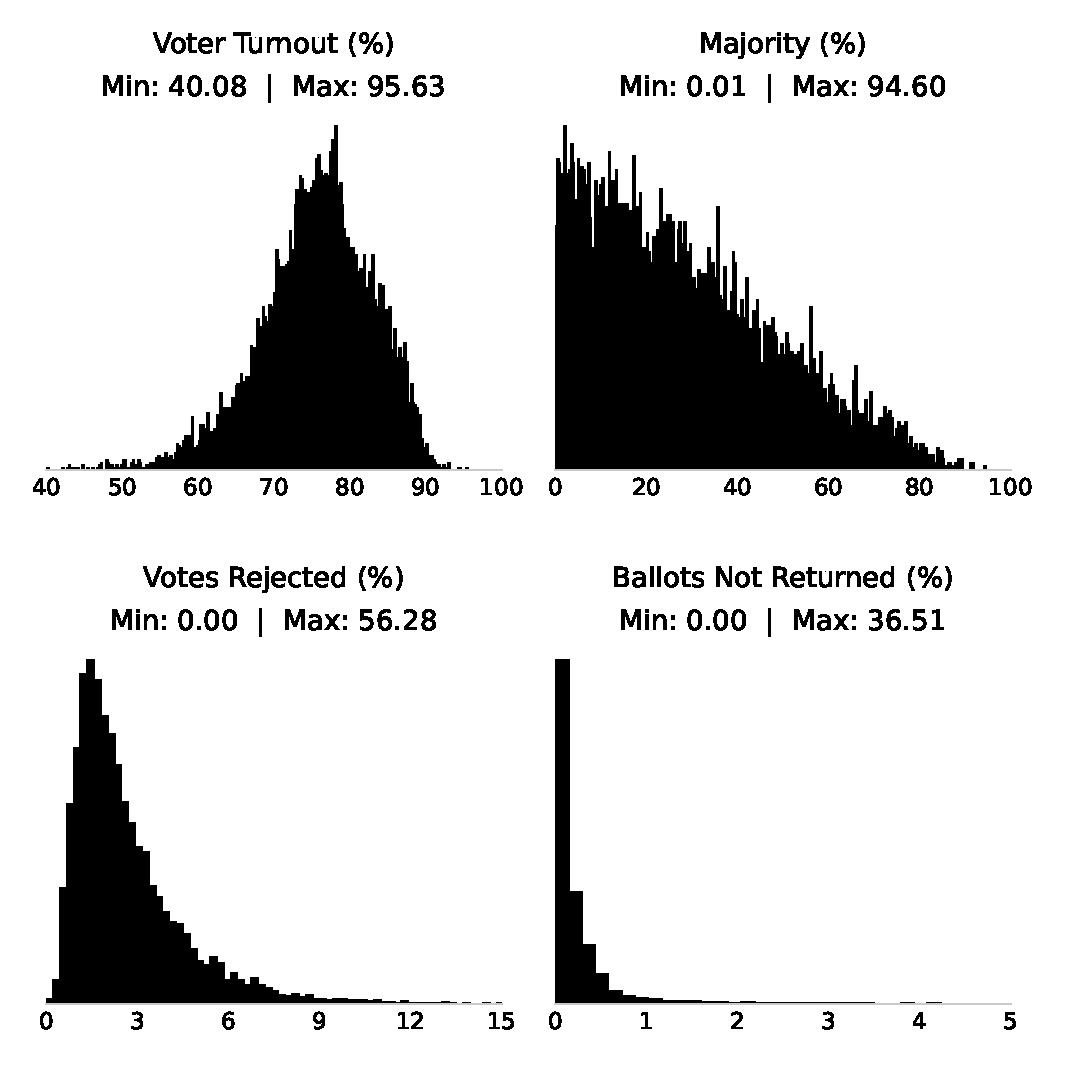
\includegraphics[width=0.8\linewidth]{dataviz/histogram_validation.eps}
	\label{fig:histograms}
\end{figure}


Wrapping up our checks on numerical values, we note that the validation procedure can fail if two errors exactly offset each other. Furthermore, it cannot detect errors in the number of registered voters, which does not enter Equation (\ref{eq:validation}). To address these limitations, we plotted histograms of 4 derived variables (Figure \ref{fig:histograms}): voter turnout rate, vote rejection rate, unreturned ballot rate, and majority as a share of valid votes. All four variables pass the check of being bounded between 0 and 100\%, and display smooth distributions as would be expected if data entry was accurate. All outlier values were double-checked; in particular, we verified that extreme instances of high rejected votes or unreturned ballots were not due to mistakes in data entry. For example, the DUN of Pangkor in Perak had two instances where over 30\% of ballots were not returned; this was due to historical inefficiencies in the implementation of postal voting for navy personnel\cite{junid2019battle}.

For non-numerical data, we conducted 3 types of checks. For parties, the full list of parties was only 100 long, so we manually checked each against publicly available information. For constituency names, we generated a list of unique constituency names (1,437 in total), which we manually checked for errors in spelling or syntax. The most challenging component was candidate names. The scale of the dataset -- \TOTALBALLOTS\space candidates across \TOTALCONTESTS\space contests -- made full manual validation infeasible. While we applied rigorous formatting standards during data entry and conducted targeted manual checks for prolific or high-profile candidates, we acknowledge that minor inconsistencies may persist. These challenges are amplified by the fact that candidates often change the spelling of their names across elections, acquire new titles and honorifics over time (e.g., Dato', Tan Sri, Haji, Ustaz, academic degrees), and format their names differently in different years (for example, omitting or reordering titles). Such variations make consistent longitudinal tracking inherently complex. As with all living datasets of this scale, we anticipate incremental improvements over time as users engage with the data and identify potential refinements.

Finally, to ensure accuracy of the database as a whole, we derive seats and votes by party for all elections in the dataset, and ensure that these match against the record of parties in Parliament and State Legislative Assemblies.
\section*{Usage Notes}

The Malaysian Election Corpus (\acronymend) is designed to support a wide range of use cases, ranging from rigorous empirical research to rapid data journalism, and even casual civic technology projects. In the academic realm, \acronym -- as the first database of its kind for Malaysia -- serves as a foundational resource for research in electoral studies, political science, and public policy. Researchers can employ the data to answer important questions about the evolution of Malaysia's electoral system, employing both cross-sectional and longitudinal analysis.

We anticipate that many users will want to extend or adapt the dataset. The standardised schema and use of lookup tables enable seamless enrichment and flexible integration with other datasets. Some valuable examples include:
\begin{enumbul}
\item \texttt{lookup\_candidates} can be enriched with data on candidates' demographic characteristics, such as age, gender, ethnic group, and education level.
\item \texttt{lookup\_parties} can be enriched with data on party affiliations, or even component parties of coalitions. For instance, by adding a \texttt{coalition} field to the lookup, it is possible to assign different UIDs to two candidates representing the same coalition, such that they can be traced to different component parties.
\item \texttt{lookup\_seats} can be enriched with a \texttt{lineage} field, which might track the geospatial lineage of a constituency, including changes in boundaries over time. However, this will require the user to define how constituency identity is determined.
\end{enumbul}
As a practical reference for users, the \texttt{dashboards.py} script illustrates how to merge the core datasets with lookup tables to create panel data suitable for interactive dashboards and advanced analyses.

Finally, while rigorous validation has been applied (see Technical Validation), this remains a living database and is intended as such. Minor inaccuracies, particularly in the candidate name field, may persist as discussed above. We encourage users to report issues or submit improvements via the GitHub repository, which provides full transparency of changes between releases. 


\section*{Code Availability}

All data processing, validation, and compilation was conducted in Python. The full source code is publicly available via \href{https://github.com/Thevesh/paper-malaysian-election-corpus}{GitHub under a CC0 license}. Three key scripts which users should find particularly useful are:

\begin{enumbul}
\item \texttt{compile.py}, which generates and validates all tabular datasets published on Harvard Dataverse, with the exception of the \texttt{lookup*.csv} files, which were manually curated.
\item \texttt{dataviz.py}, which generates all visualisations used in this paper.
\item \texttt{dashboards.py}, which generates the source files for the interactive visualisations available at \href{https://electiondata.my}{ElectionData.MY}.
\end{enumbul}

% this section generates reference
\begingroup
\raggedright
\linespread{1.1}
\small
\let\oldthebibliography\thebibliography
\bibliography{mybib}
\endgroup

\section*{Author Contributions}
TT conceived, designed, and carried out all aspects of this study, including data collection, data curation, analysis, and manuscript preparation.

\section*{Competing Interests}
The author declares no competing interests. The author is not affiliated with any political party, or any organization which actively participates in or aims to influence the outcome of Malaysian elections.

\section*{Acknowledgements}
This work did not receive any specific funding. We thank Rosmadi Fauzi and Zulkanain Abdul Rahman for their helpful feedback and suggestions on the dataset and manuscript. We also gratefully acknowledge Nimesha Thevananthan for their assistance with data collection, as well as Danesh Prakash Chacko of Tindak Malaysia for providing historical insights and filling data gaps, particularly for the Sabah state election in 1971. Finally, we thank the EC for granting access to physical records of historical election results via \textit{Pusat Sumber SPR}.

\end{document}